\documentclass[12pt,utf8]{beamer}

% Gute Einführung zu LaTeX-Beamer: http://www2.informatik.hu-berlin.de/~mischulz/beamer.html

%-----PARAMETERS-----

%Wichtige Standard Pakete!
%\usepackage[german]{babel}
\usepackage{ngerman}
\usepackage{xcolor}
\usepackage{graphicx}
\usepackage{tikz}

%Für den Header notwendig!
%\usepackage[percent]{overpic}

\usepackage{hyperref} % für korrekte Links

%Einbinden des Themes
\input{design_latex-template/beamerthemeFOSSAG.sty}


%Standard Angaben
\title{
	\hspace*{8cm}
	
\includegraphics[scale=0.2]{resources/logo_500px.png}
	\newline
	FOSS-AG
}
\subtitle{Tensorflow - Workshop}
%\author{@chef\_excellence}
\institute[FOSS AG]{\textbf{F}ree and \textbf{O}pen \textbf{S}ource \textbf{S}oftware \textbf{AG}}

\date{29. Mai 2018}

%-----IMPLEMENTATION-----
\begin{document}
	\begin{frame}
		\titlepage
	\end{frame}

	\begin{frame}
		\centering Was ist Machine Learning?
	\end{frame}

	\begin{frame}
		\centering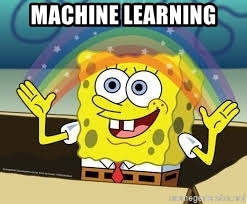
\includegraphics[scale=1]{resources/machine-learning.jpg}\\
		{\tiny Source: \cite{memegen}}
	\end{frame}

	\begin{frame}
		\frametitle{Was ist Machine Learning?}
		\begin{itemize}
			\item Lernen/Schätzen von Eigenschaft eines Datensatzes mittels statistischer Verfahren
			\item Generalisierung von Lerndaten auf Gesamtmenge
		\end{itemize}
	\end{frame}
	
	\begin{frame}
		\frametitle{Machine Learning - Probleme}
		\begin{itemize}
			\item Klassifikation / Clustering
			\item Regression
			\item Prognosen / Vorhersagen
			\item Synthese
		\end{itemize}
	\end{frame}
	
	\begin{frame}
		\frametitle{Machine Learning - Probleme}
		\begin{itemize}
			\item Klassifikation / Clustering
			\item \textcolor{black!20}{Regression}
			\item\textcolor{black!20}{Prognosen / Vorhersagen}
			\item \textcolor{black!20}{Synthese}
		\end{itemize}
	\end{frame}
	
	\begin{frame}
		\frametitle{Machine Learning - Modelle}
		\begin{itemize}
			\item Support Vector Machines
			\item Artificial Neural Networks
			\item Random Markov Fields
			\item k-Nearest Neighbors
		\end{itemize}
	\end{frame}	
	
	\begin{frame}
		\frametitle{Machine Learning - Modelle}
		\begin{itemize}
			\item \textcolor{black!20}{Support Vector Machines}
			\item Artificial Neural Networks
			\item \textcolor{black!20}{Random Markov Fields}
			\item \textcolor{black!20}{k-Nearest Neighbors}
		\end{itemize}
	\end{frame}
	
	\begin{frame}
		\centering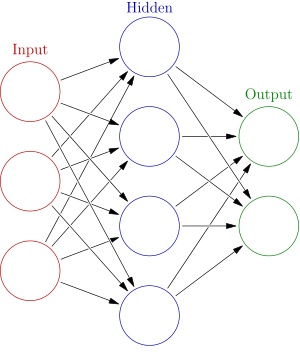
\includegraphics[scale=0.5]{resources/300px-Colored_neural_network.png}\\
		{\tiny Source: \cite{ann_wiki} (CC BY-SA 3.0)}
	\end{frame}
	
	\begin{frame}
		\frametitle{Artificial Neural Networks}
		
	\end{frame}
	
	\begin{frame}
		\bibliographystyle{plain}
		\bibliography{literatur}
		\addcontentsline{toc}{section}{\bibname}
	\end{frame}

\end{document}
